\documentclass[conference]{IEEEtran}
\usepackage{cite}
\usepackage{amsmath,amssymb,amsfonts}
\usepackage{algorithmic}
\usepackage{graphicx}
\usepackage{textcomp}
\usepackage{xcolor}
\usepackage{listings}
\usepackage{enumitem}
\usepackage{multirow}
\usepackage{url}

\begin{document}

\title{HealthHub: A Comprehensive Health Data Management Platform with RAG-Enhanced AI Analysis}

\author{\IEEEauthorblockN{Author Name}
\IEEEauthorblockA{\textit{Department of Information Science and Engineering} \\
\textit{RV College of Engineering}\\
Bengaluru, India \\
email@rvce.edu.in}}

\maketitle

\begin{abstract}
This paper presents HealthHub, an AI-powered personal health assistant designed to help individuals make informed daily dietary choices by providing personalized food safety and nutritional insights. Users can log food intake, which HealthHub analyzes using a Retrieval-Augmented Generation (RAG) pipeline to query diverse sources like FSSAI advisories and food databases, and an SQL agent for nutritional pattern analysis. The system uniquely integrates personal health sensor data (e.g., heart rate) to correlate diet with physiological responses, offering potential risk warnings. HealthHub features an intuitive voice and video-enabled interface, aiming to empower users with accessible, actionable information for enhanced food safety awareness and personal well-being. Performance evaluations highlight the system's capability in processing user queries effectively and integrating multimodal data for comprehensive dietary support.
\end{abstract} 
% Chapter 1: Introduction to IoT-Based Vital Sign Monitoring System with Conversational Health Data Access
% This section should contain the use of the project in real time, as per the provided guidelines.

\section*{Introduction}
Your introduction content goes here.

\section{Background}

\subsection{Retrieval-Augmented Generation}
RAG combines information retrieval with language model generation to provide context-aware responses [9]. In healthcare applications, RAG addresses several key challenges [1]:

\begin{itemize}
\item \textbf{Context Preservation:} Ensures responses are grounded in relevant medical documentation
\item \textbf{Accuracy:} Reduces hallucination by providing source material
\item \textbf{Verifiability:} Enables tracking of information sources
\item \textbf{Customization:} Allows adaptation to specific medical contexts
\end{itemize}

\subsection{SQL Agents in Healthcare}
SQL agents provide natural language interfaces to structured databases [14]. Their application in healthcare offers several advantages [4]:

\begin{itemize}
\item \textbf{Accessibility:} Enables natural language queries of sensor data
\item \textbf{Real-time Analysis:} Facilitates immediate access to sensor readings
\item \textbf{Data Integration:} Connects multiple sensor data sources
\item \textbf{Automated Insights:} Generates human-readable interpretations of sensor data
\end{itemize}

\subsection{Vector Databases in Healthcare}
Vector databases play a crucial role in modern healthcare systems [2]:

\begin{itemize}
\item \textbf{Semantic Search:} Enables meaning-based document retrieval
\item \textbf{Similarity Matching:} Identifies related medical records
\item \textbf{Efficient Retrieval:} Provides fast access to relevant information
\item \textbf{Scalability:} Handles large volumes of medical documents
\end{itemize}

\subsection{Related Work}
Previous research in healthcare data management has explored various approaches [5, 6]:

\begin{itemize}
\item Traditional document retrieval systems lacking context awareness
\item Natural language interfaces with limited integration capabilities
\item Sensor data management systems without AI-powered querying
\item Standalone RAG implementations without sensor data integration
\end{itemize}

HealthHub builds upon these foundations while addressing their limitations through the novel integration of RAG and SQL agent technologies [11]. 
\section{METHODOLOGY}

\subsection{Implementation Tasks}

\begin{enumerate}

\item \textbf{Frontend Development}
\begin{itemize}
    \item Design the user interface using \textbf{Next.js} with \textbf{TailwindCSS} and \textbf{shadcn/ui} for a responsive, modular experience.
    \item Build a real-time dashboard to visualize health metrics such as SpO2, heart rate, ECG, and temperature.
    \item Integrate Supabase Auth to enable secure user login and session handling.
\end{itemize}

\item \textbf{Backend Development}
\begin{itemize}
    \item Set up a \textbf{FastAPI} server to handle incoming sensor data and expose RESTful endpoints.
    \item Use a \textbf{PostgreSQL} database (hosted via Supabase) to store and manage health data securely.
    \item Develop APIs for data submission, retrieval, and query handling.
\end{itemize}

\item \textbf{IoT Sensor Integration}
\begin{itemize}
    \item Use an \textbf{Arduino UNO R3} to interface with all biomedical sensors and read analog/digital inputs.
    \item Employ an \textbf{ESP8266 Wi-Fi module} to transmit data to the cloud via HTTP or MQTT.
    \item Configure periodic data sampling and preprocessing before cloud transmission.
\end{itemize}

\item \textbf{AI Integration}
\begin{itemize}
    \item Integrate a conversational AI interface using \textbf{LangChain} and \textbf{GPT-4/GPT-4o}.
    \item Allow users to query their health records through natural language using a Text-to-SQL pipeline.
    \item Provide automated health summaries and anomaly detection powered by AI.
\end{itemize}

\end{enumerate}

\section{Implementation}

\subsection{System Architecture}
The HealthHub platform implements a modern microservices architecture [3]:

\begin{itemize}
\item \textbf{Frontend Layer:}
    \begin{itemize}
    \item Next.js 14 application with App Router
    \item Server-side rendering for performance
    \item Real-time data updates via WebSocket
    \item Responsive design with Tailwind CSS
    \end{itemize}

\item \textbf{Backend Services:}
    \begin{itemize}
    \item FastAPI service for RAG pipeline
    \item Supabase for real-time data and authentication
    \item PostgreSQL with pgvector extension
    \item LangChain for AI orchestration
    \end{itemize}
\end{itemize}

\subsection{RAG Pipeline Architecture}
\begin{figure}[!t]
\centering
\includegraphics[width=\columnwidth]{figures/rag-architecture}
\caption{RAG Pipeline Implementation for Medical Records}
\label{fig:rag-architecture}
\end{figure}

The RAG pipeline processes medical records through a series of steps identified in recent literature [10, 7]:
\begin{itemize}
\item Document chunking and preprocessing
\item Cohere embedding generation
\item Vector storage in Supabase
\item Context-aware query processing
\end{itemize}

\subsection{SQL Agent Architecture}
\begin{figure}[!t]
\centering
\includegraphics[width=\columnwidth]{figures/sql-agent-flow}
\caption{SQL Agent Query Processing Flow}
\label{fig:sql-agent-flow}
\end{figure}

Building on recent advances in natural language to SQL conversion [14, 15], the SQL agent handles sensor data through:
\begin{itemize}
\item Natural language query parsing
\item Automated SQL query generation
\item Real-time data retrieval
\item Response formatting and visualization
\end{itemize}

\subsection{Integration Layer}
The system integrates these components through:
\begin{itemize}
\item Unified API gateway
\item Shared authentication system
\item Common data access layer
\item Centralized error handling
\end{itemize}

\begin{figure}[!t]
\centering
\includegraphics[width=\columnwidth]{figures/system-integration}
\caption{System Integration Architecture}
\label{fig:system-integration}
\end{figure} 
\section{Results}

This section presents the key outcomes from the development and initial testing of the HealthHub platform. We focused on evaluating the core functionalities, user interface effectiveness, and the performance of the AI-driven food safety and nutritional analysis features, particularly those concerning FSSAI guidelines and personal health data.

\subsection{User Interface and Experience}
HealthHub provides a clean and intuitive user interface, designed to make complex health and food safety information accessible. Figure \ref{fig:hm-hero} showcases the platform's landing page, introducing users to HealthHub's capabilities.

\begin{figure}[!t]
\centering
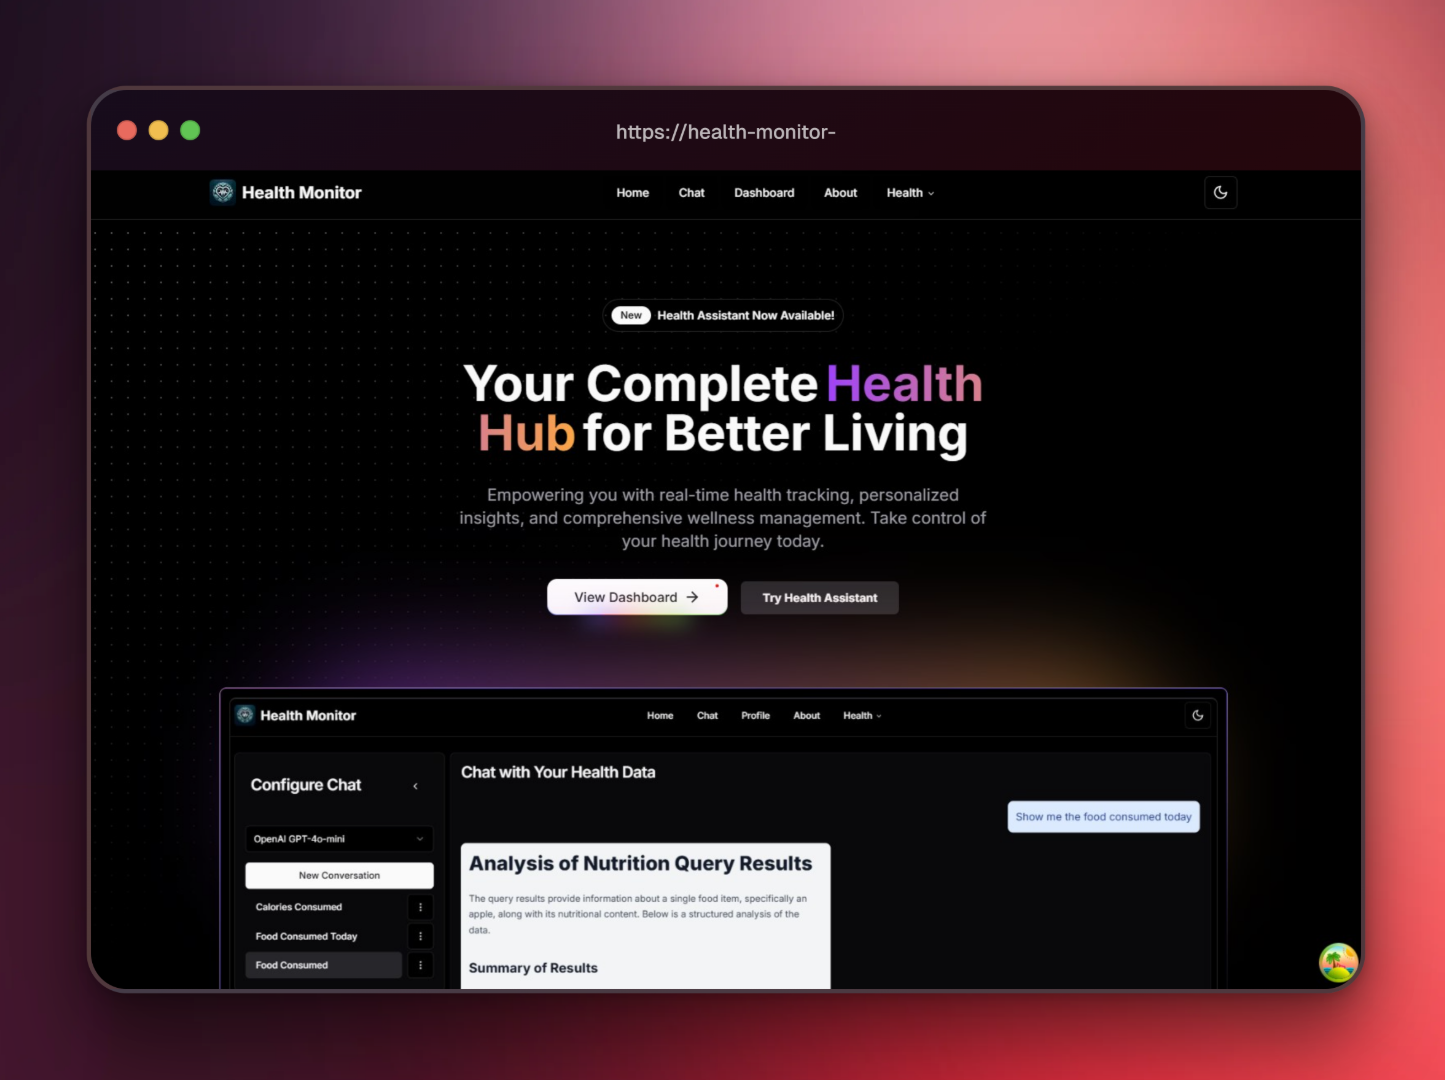
\includegraphics[width=0.9\columnwidth]{figures/hm-hero.png} % User to confirm/update path
\caption{The HealthHub landing page, highlighting its core features and value proposition to the user.}
\label{fig:hm-hero}
\end{figure}

Upon logging in, users are presented with the main dashboard (Figure \ref{fig:hm-dashboard}), which offers an overview of their logged data and quick access to various features, including food logging and initiating queries.

\begin{figure}[!t]
\centering
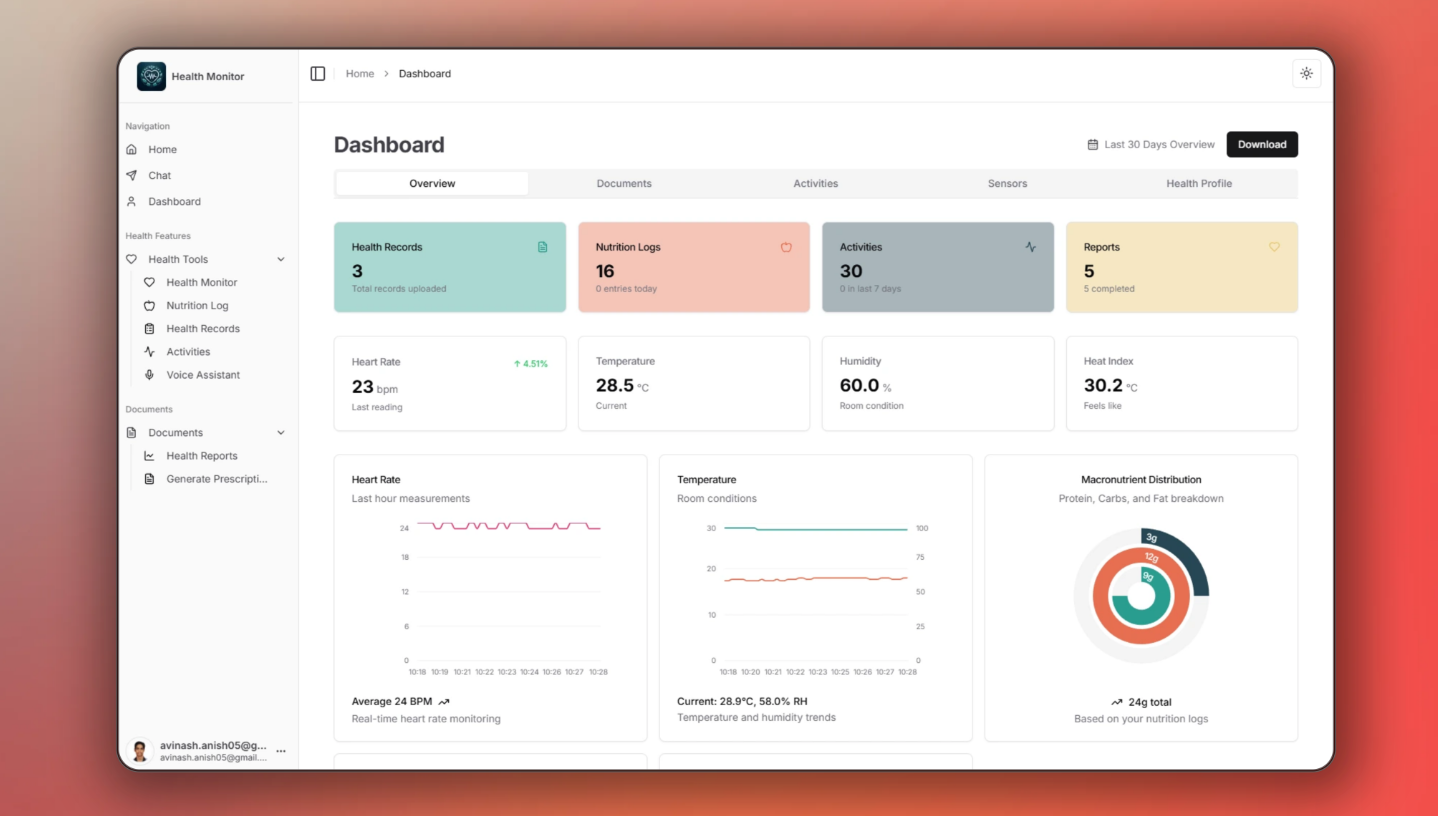
\includegraphics[width=0.9\columnwidth]{figures/hm-dashboard.png} % User to confirm/update path
\caption{The HealthHub main dashboard, providing a central point for users to view their health summary and access features.}
\label{fig:hm-dashboard}
\end{figure}

HealthHub supports multiple modalities for interacting with its AI assistant. Figure \ref{fig:hm-chat} illustrates the text-based chat interface. Furthermore, an integrated AI Voice and Video Assistant, shown in Figure \ref{fig:hm-video-assistant}, allows users to engage in spoken conversations and receive visual feedback from an AI avatar, enhancing the interactive experience.

\begin{figure}[!t]
\centering
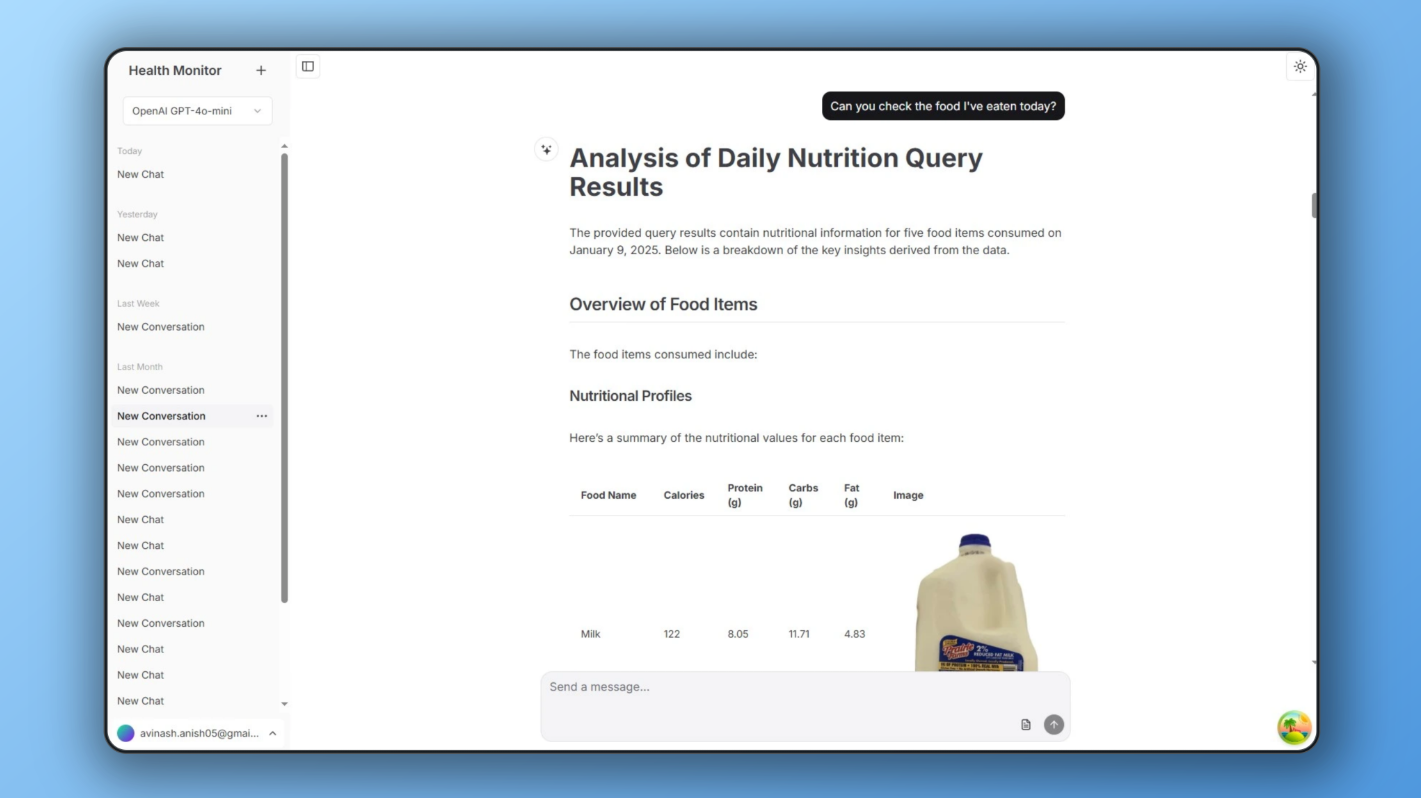
\includegraphics[width=0.9\columnwidth]{figures/hm-chat.png} % User to confirm/update path
\caption{HealthHub's text chat interface for querying the AI assistant about food safety, FSSAI guidelines, and nutrition.}
\label{fig:hm-chat}
\end{figure}

\begin{figure}[!t]
\centering
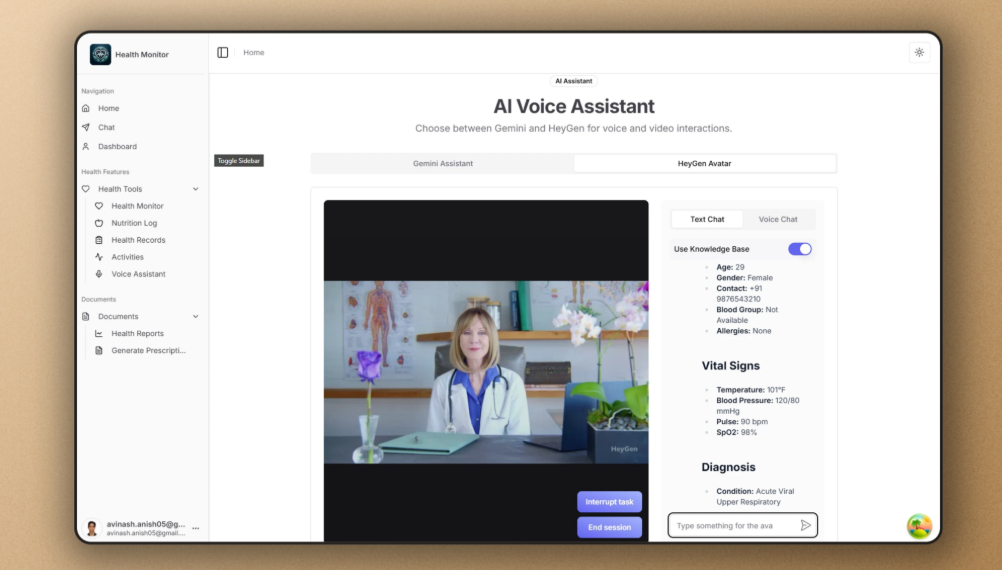
\includegraphics[width=0.8\columnwidth]{figures/hm-video.png} % Changed from 0.7, user to confirm filename (hm-video.png or specific AI assistant image)
\caption{The HealthHub AI Voice and Video Assistant interface, enabling spoken interaction and visual feedback.}
\label{fig:hm-video-assistant}
\end{figure}

\subsection{AI-Powered Food Safety and Nutritional Analysis}
Our AI core, combining a RAG pipeline and an SQL agent, demonstrated its ability to provide relevant and personalized information. Table \ref{tab:rag-examples} presents illustrative examples of the RAG pipeline addressing FSSAI and food safety queries.

\begin{table}[!ht]
\centering
\caption{Illustrative FSSAI & Food Safety Queries (RAG Pipeline)}
\label{tab:rag-examples}
\begin{tabular}{|p{0.4\columnwidth}|p{0.5\columnwidth}|}
\hline
\textbf{User Query/Scenario} & \textbf{HealthHub Response (Illustrative)} \\
\hline
User types: "Are there FSSAI rules for using artificial sweeteners in baked goods?" & Yes, FSSAI's Food Safety and Standards (Food Products Standards and Food Additives) Regulations, 2011, specify approved artificial sweeteners like Aspartame and Sucralose for use in baked goods, within prescribed maximum limits. For example, Aspartame is permitted up to 1000 mg/kg in certain bakery products. It's important to check product labels for declarations. \\
\hline
User asks: "What does FSSAI say about pesticide residues in fruits?" & FSSAI has established Maximum Residue Limits (MRLs) for various pesticides in different food commodities, including fruits, under the Food Safety and Standards (Contaminants, Toxins and Residues) Regulations, 2011. These limits are regularly reviewed. For specific fruits, it's best to refer to the latest FSSAI notifications on MRLs. \\
\hline
\end{tabular}
\end{table}

Table \ref{tab:sql-agent-examples} showcases the SQL agent processing natural language queries against logged dietary data.

\begin{table}[!ht]
\centering
\caption{Illustrative Personalized Nutritional Insights (SQL Agent)}
\label{tab:sql-agent-examples}
\begin{tabular}{|p{0.4\columnwidth}|p{0.5\columnwidth}|}
\hline
\textbf{User Query/Scenario} & \textbf{HealthHub Response (Illustrative)} \\
\hline
User asks via voice: "HealthHub, what was my average daily sugar intake this past week?" & Based on your logged food items from the past week, your average daily sugar intake was approximately 65 grams. The World Health Organization recommends adults consume no more than 25-50 grams of free sugars per day for optimal health. \\
\hline
User types: "Compare my protein intake yesterday with the day before." & Yesterday, your protein intake was 70g. The day before, it was 55g. You consumed 15g more protein yesterday. \\
\hline
\end{tabular}
\end{table}

\subsection{Sensor Data Integration and Alert Potential}
The sensor subsystem successfully logged physiological data (e.g., heart rate, SpO2 from MAX30102) to the user's profile. This data enables correlational analysis, as illustrated in Table \ref{tab:sensor-alert-example}.

\begin{table}[!ht]
\centering
\caption{Illustrative Sensor Data Correlation and Advisory}
\label{tab:sensor-alert-example}
\begin{tabular}{|p{0.4\columnwidth}|p{0.5\columnwidth}|}
\hline
\textbf{System Trigger/Scenario} & \textbf{HealthHub Advisory (Illustrative)} \\
\hline
User logs consumption of a highly caffeinated energy drink. System correlates this with sensor data showing a heart rate increase from baseline 70 bpm to 105 bpm, sustained for 45 minutes. & Noticed a significant heart rate increase after your logged energy drink. Frequent high caffeine intake can impact cardiovascular health. Consider moderation. \\
\hline
\end{tabular}
\end{table}

\subsection{System Performance and Responsiveness}
Initial evaluations indicate that HealthHub is responsive. Queries to the RAG pipeline for FSSAI information were typically answered within 3-5 seconds. The SQL agent also demonstrated efficient query execution for nutritional summaries, usually taking less than 2 seconds. While formal benchmarking is ongoing, the current performance supports an engaging user experience. 
\section{Conclusion}

This paper introduced HealthHub, an AI-powered personal health assistant designed to empower individuals with accessible and actionable information regarding food safety and nutrition, with a particular focus on leveraging FSSAI guidelines and integrating personal sensor data. We have detailed its architecture, core AI components—a Retrieval-Augmented Generation (RAG) pipeline for contextual food safety information and an SQL agent for personalized dietary and sensor data analysis—and its user-centric multi-modal interface featuring chat, voice, and video interactions.

Our work demonstrates the successful development of a platform with key capabilities:
\begin{itemize}
    \item Effective processing of user queries regarding FSSAI standards and food content through its RAG pipeline.
    \item Provision of personalized nutritional summaries via its SQL agent.
    \item Successful logging of physiological data from wearable sensors.
    \item Delivery of relevant information and illustrative advisories based on integrated food, FSSAI, and sensor data, aiming to bridge the gap between complex safety information and the consumer.
\end{itemize}

While HealthHub presents a promising approach, we acknowledge certain limitations:
\begin{itemize}
    \item The RAG pipeline's current knowledge base, while substantial, covers a subset of the extensive FSSAI regulations and requires continuous expansion and updates.
    \item Insights from sensor data correlations are observational and intended for user awareness, not as a substitute for professional medical advice.
    \item The current performance evaluation is based on initial tests; formal benchmarking and extensive real-world user testing are important next steps.
\end{itemize}

Future work will concentrate on several key areas to enhance HealthHub's capabilities and impact:
\begin{itemize}
    \item \textbf{Knowledge Base Expansion:} Continuously updating and broadening the FSSAI and food safety knowledge base to include more products, regional variations, and emerging safety concerns.
    \item \textbf{AI Model Enhancements:} Improving the nuanced understanding of user queries by the AI models and developing predictive analytics based on long-term dietary and sensor data trends.
    \item \textbf{Advanced Alert Mechanisms:} Designing and implementing more sophisticated, context-aware, and potentially clinically validated alert systems.
    \item \textbf{User Studies and Iteration:} Conducting comprehensive user studies to gather feedback for iterative refinement of the platform's features and usability.
    \item \textbf{Mobile Application Development:} Exploring the creation of a dedicated mobile application to improve accessibility and user engagement.
\end{itemize}

In conclusion, HealthHub offers a novel integration of AI technologies to address the critical need for personalized food safety and health guidance. By making complex information more understandable and actionable, it holds the potential to contribute significantly to individual well-being and informed consumer choices. 

% References section
\begin{thebibliography}{16}
[1] M. Alkhalaf, P. Yu, M. Yin, and C. Deng, "Applying generative AI with 
    retrieval-augmented generation to summarize and extract key clinical 
    information from electronic health records," Journal of Biomedical 
    Informatics, p. 104662, 2024.

[2] T. Searle, Z. Ibrahim, J. Teo, and R. J. B. Dobson, "Discharge summary 
    hospital course summarization of inpatient electronic health record text 
    with clinical concept-guided deep pre-trained transformer models," Journal 
    of Biomedical Informatics, p. 104358, 2023.

[3] S. Sai et al., "Generative AI for transformative healthcare: A comprehensive 
    study of emerging models, applications, case studies, and limitations," IEEE 
    Access, vol. 12, pp. 31078-31106, 2024.

[4] S. Reddy, "Generative AI in healthcare: An implementation science-informed 
    translational path on application, integration, and governance," 
    Implementation Science, vol. 19, p. 27, 2024.

[5] P. Zhang and M. N. Kamel Boulos, "Generative AI in medicine and healthcare: 
    Promises, opportunities, and challenges," Future Internet, vol. 15, no. 9, 
    p. 286, 2023.

[6] "Leveraging generative AI models for synthetic data generation in healthcare: Balancing research and privacy," in 2023 International Conference on Smart Applications, Communications and Networking (SmartNets), 2023.

[7] W. Saba, S. Wendelken, and J. Shanahan, "Question-answering-based summarization of electronic health records using retrieval-augmented generation," arXiv preprint arXiv:2401.01469, 2024.

[8] "Redefining medicine: The power of generative AI in modern healthcare," in 2024 5th International Conference on Smart Electronics and Communication (ICOSEC), 2024.

[9] D. S. W. Ting et al., "Retrieval-augmented generation for large language models and its generalizability in assessing medical fitness," arXiv preprint arXiv:2410.08431, 2024.

[10] L. M. Amugongo et al., "Retrieval-augmented generation for large language models in healthcare: A systematic review," Preprints, 2024.

[11] A. Bora and H. Cuayáhuitl, "Systematic analysis of retrieval-augmented generation-based LLMs for medical chatbot applications," Machine Learning and Knowledge Extraction, vol. 6, pp. 2355–2374, 2024.

[12] E. Albaroudi, T. Mansouri, and A. Alameer, "The intersection of generative AI and healthcare: Addressing challenges to enhance patient care," in 2024 Seventh International Women in Data Science Conference (WiDS PSU), 2024.

[13] Y. Xu, "The investigation of the application of RAG technology in the field of EHR," Science and Technology of Engineering, Chemistry and Environmental Protection, 2024.

[14] C. Troy, S. Sturley, J. M. Alcaraz-Calero, and Q. Wang, "Enabling generative AI to produce SQL statements: A framework for the auto-generation of knowledge based on EBNF context-free grammars," IEEE Access, vol. 11, pp. 123543-123564, 2023.

[15] P. Omrani et al., "Hybrid retrieval-augmented generation approach for LLMs query response enhancement," in 2024 10th International Conference on Web Research (ICWR), 2024.

[16] G. Papanastasiou, N. Dikaios, J. Huang, C. Wang, and G. Yang, "Is attention all you need in medical image analysis? A review," IEEE Journal of Biomedical and Health Informatics, vol. 28, no. 3, pp. 1398-1411, 2024.
\end{thebibliography}

\end{document} 